\documentclass[
size=17pt,
paper=smartboard,
mode=present,
display=slidesnotes,
style=paintings,
nopagebreaks,
blackslide,
fleqn]{powerdot}

% styles: sailor, paintings
% wj capsules prettybox
% mode = handout or present


\usepackage{amsmath,graphicx,color,amsfonts}
\usepackage[brazilian]{babel}
\usepackage[utf8]{inputenc}
\newcommand{\palette}{Moitessier}


% palettes:
%    - sailor: Sea, River, Wine, Chocolate, Cocktail 
%    - paintings: Syndics, Skater, GoldenGate, Moitessier, PearlEarring, Lamentation, HolyWood, Europa, MayThird, Charon 

\newcommand{\cursopequeno}{EC01039 CG\underline{PI}}
\newcommand{\cursogrande}{\Large EC01039 -- Computação gráfica e \underline{processamento de imagem}}



\author{Ronaldo de Freitas Zampolo\\FCT-ITEC-UFPA}
\date{2020.2}


\pdsetup{
	lf = {\cursopequeno},
	rf = {Sensores e aquisição}, 
	cf = {\arabic{slide}~/~\pageref*{lastslide}},
	palette = {\palette}, 
	randomdots={false}
}

%opening
\title{\cursogrande\\ \vspace{1cm}Sensores e aquisição de imagens}
\author{Ronaldo de Freitas Zampolo\\FCT-ITEC-UFPA}
%\date{ }

\begin{document}
   \maketitle[randomdots={false}]
   \begin{slide}{Agenda}
      \tableofcontents[content=sections]
   \end{slide}

\section[ slide = true ]{Sensores e aquisição de imagens}
   \begin{slide}[toc=]{Foto sensores}
      \begin{itemize}[type=1]
         \item Sensor: converte energia luminosa em corrente/tensão elétrica
         \item Arranjos de sensores
         \begin{center}
               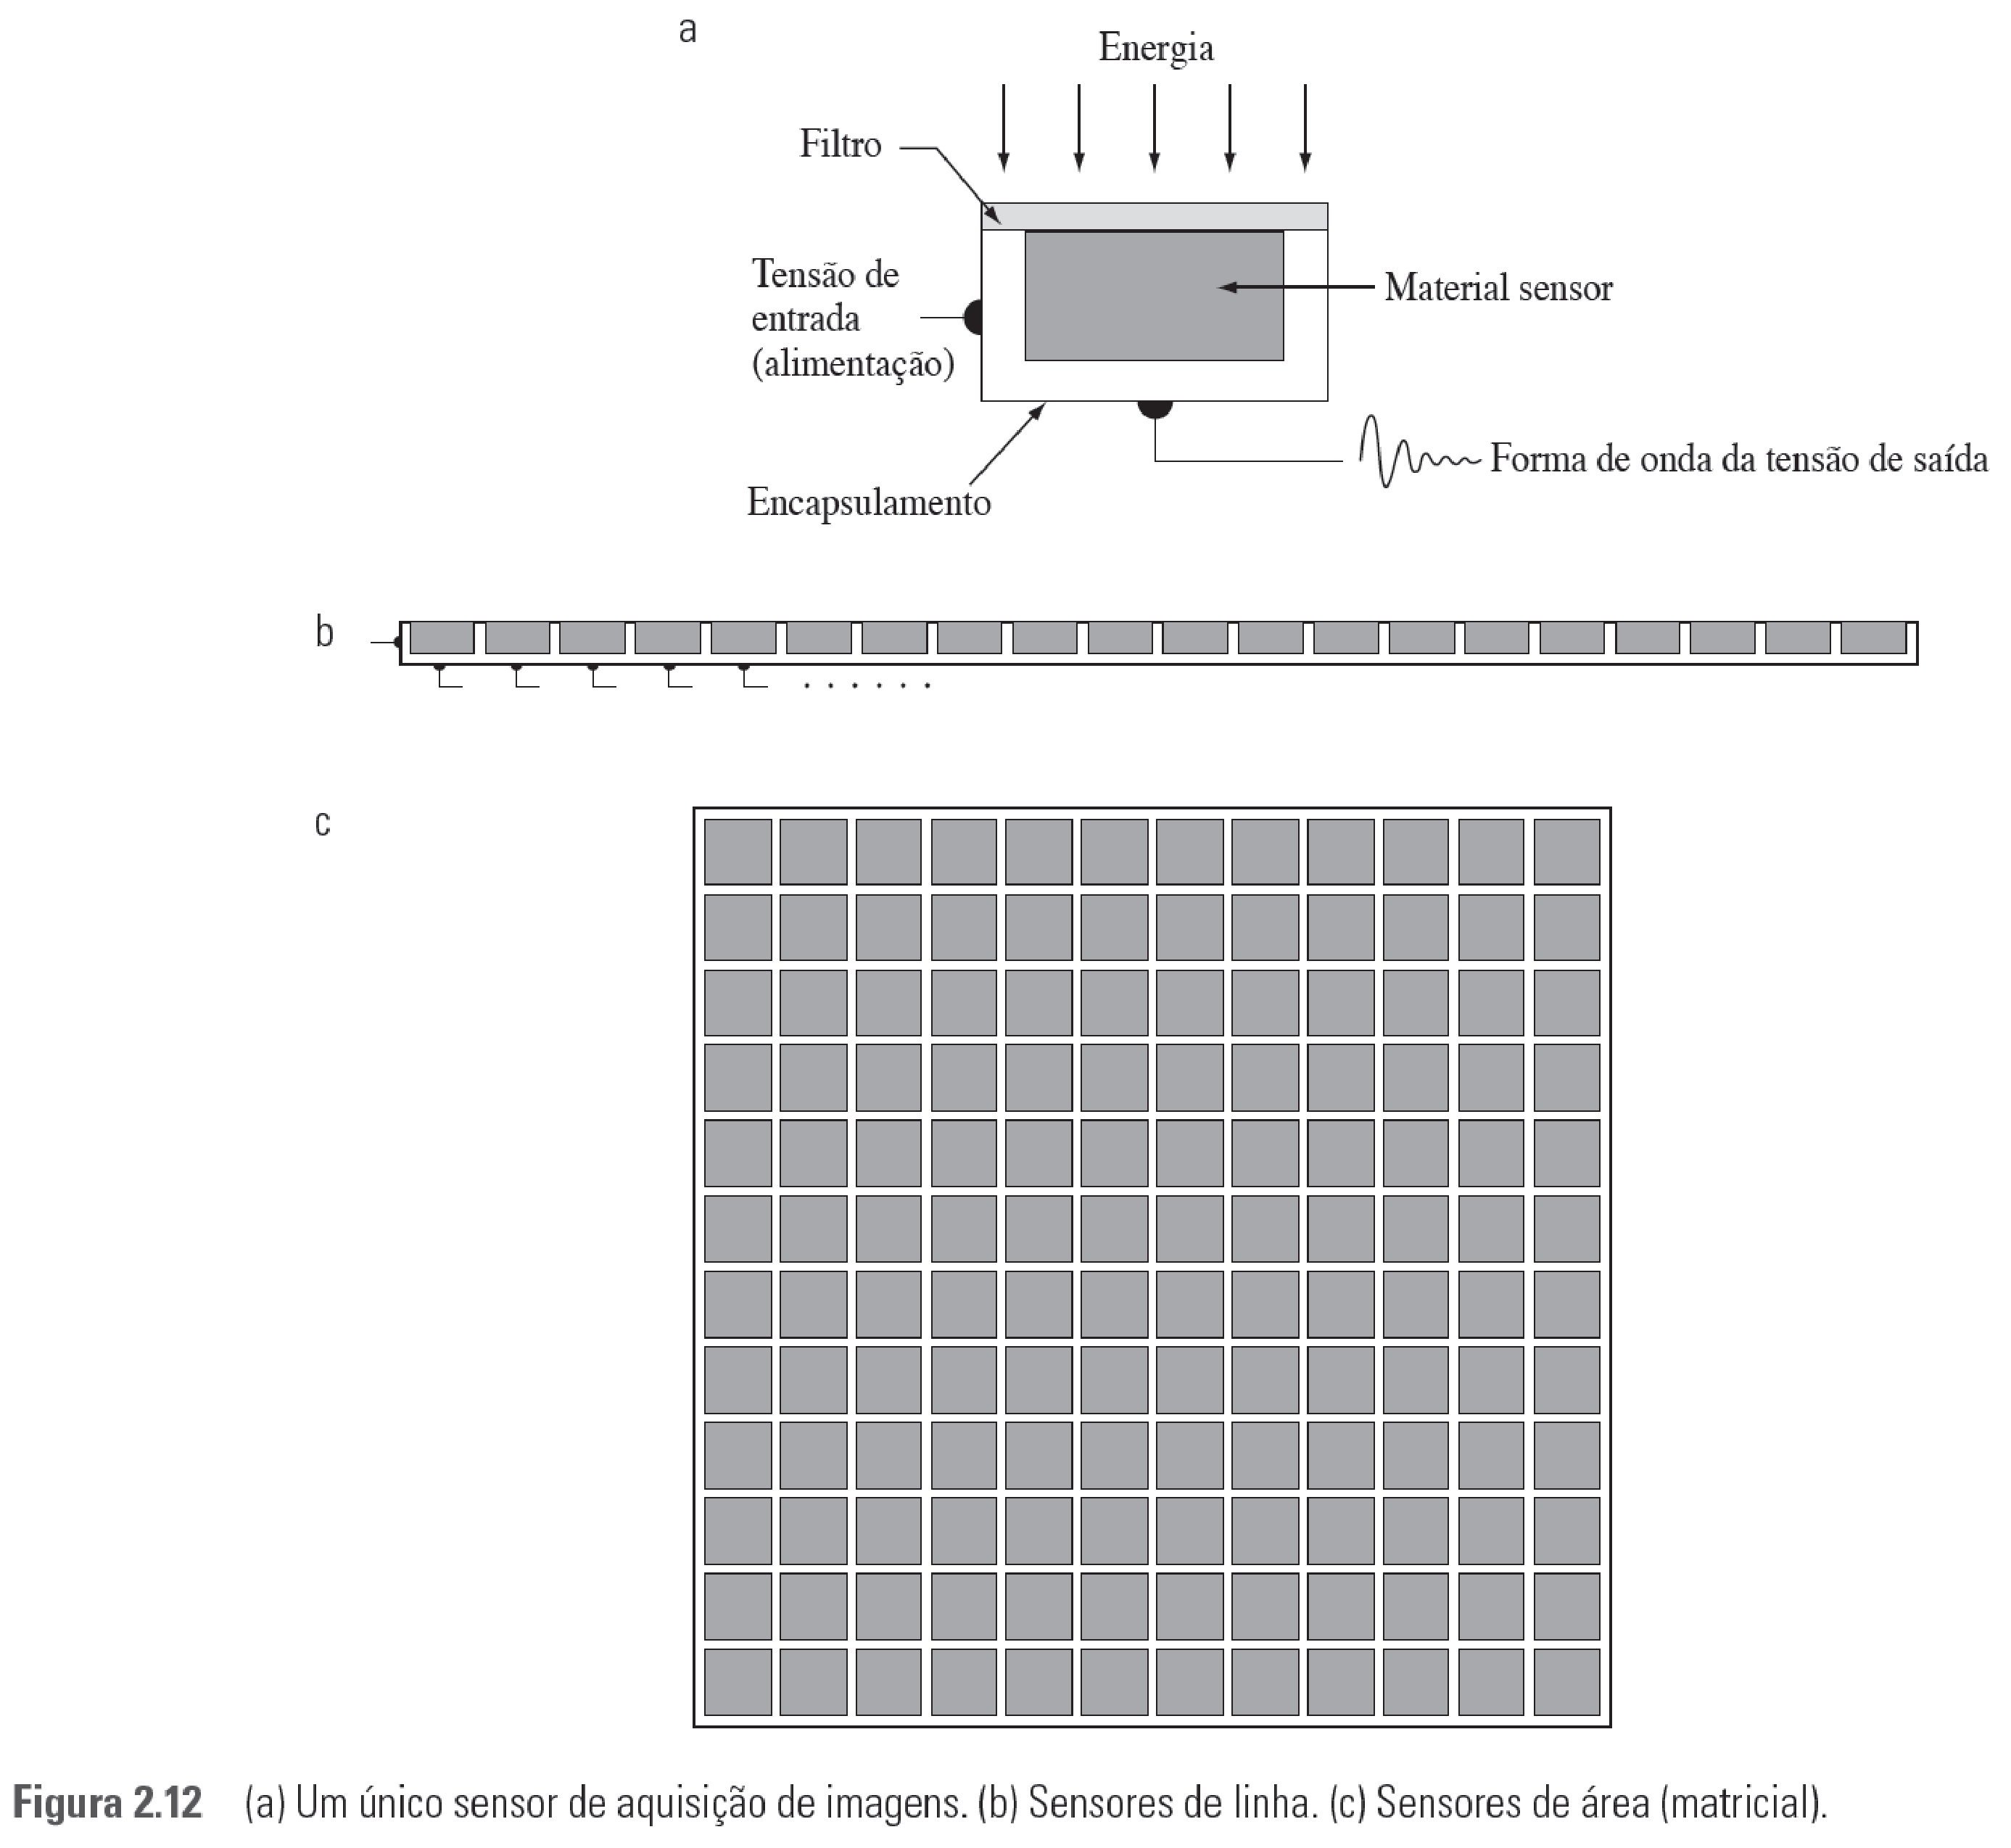
\includegraphics[width=0.5\textwidth]{figs/fig0212}
            \end{center}
      \end{itemize}
   \end{slide}

   \begin{slide}[toc=]{Arranjos de foto sensores}
      \begin{itemize}[type=1]
         \item Um único sensor
            \begin{center}
               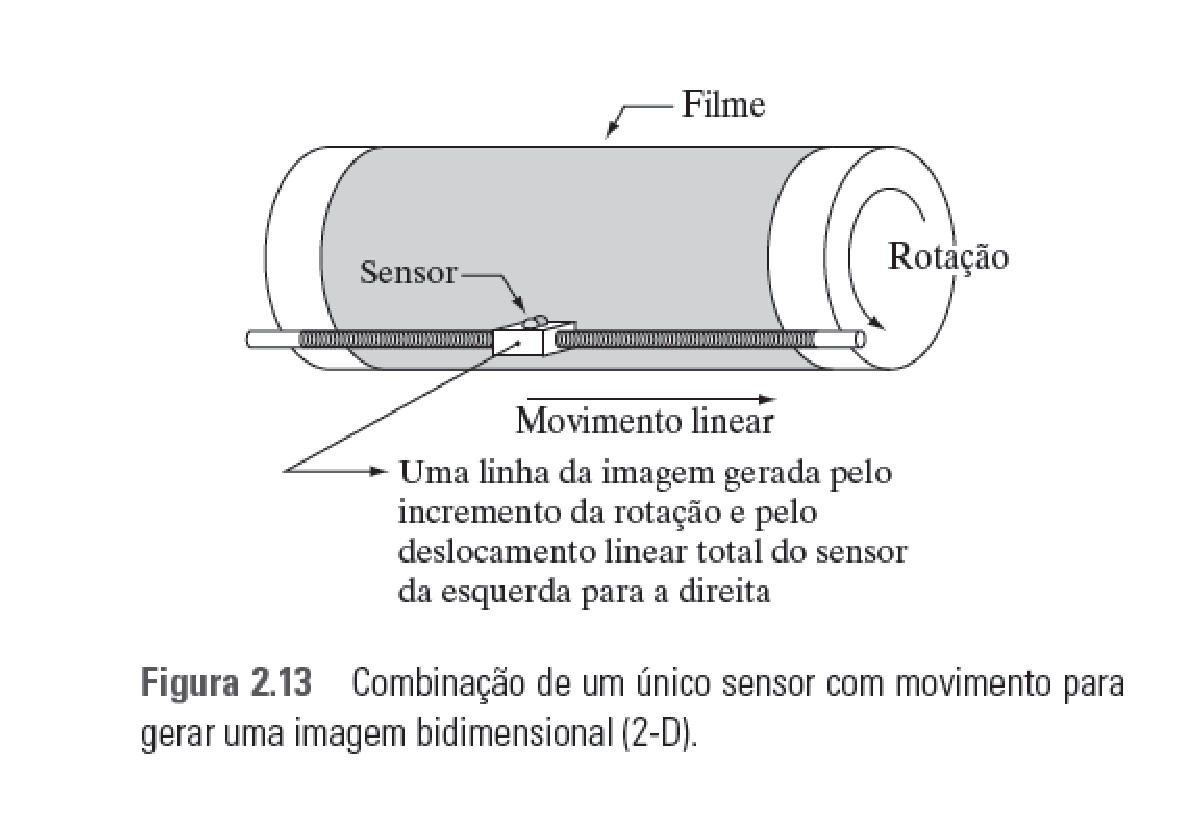
\includegraphics[width=0.7\textwidth]{figs/fig0213}
            \end{center}
      \end{itemize}
   \end{slide}
   
   \begin{slide}[toc=]{Arranjos de foto sensores}
      \begin{itemize}[type=1]
         \item Sensores em linha
            \begin{center}
               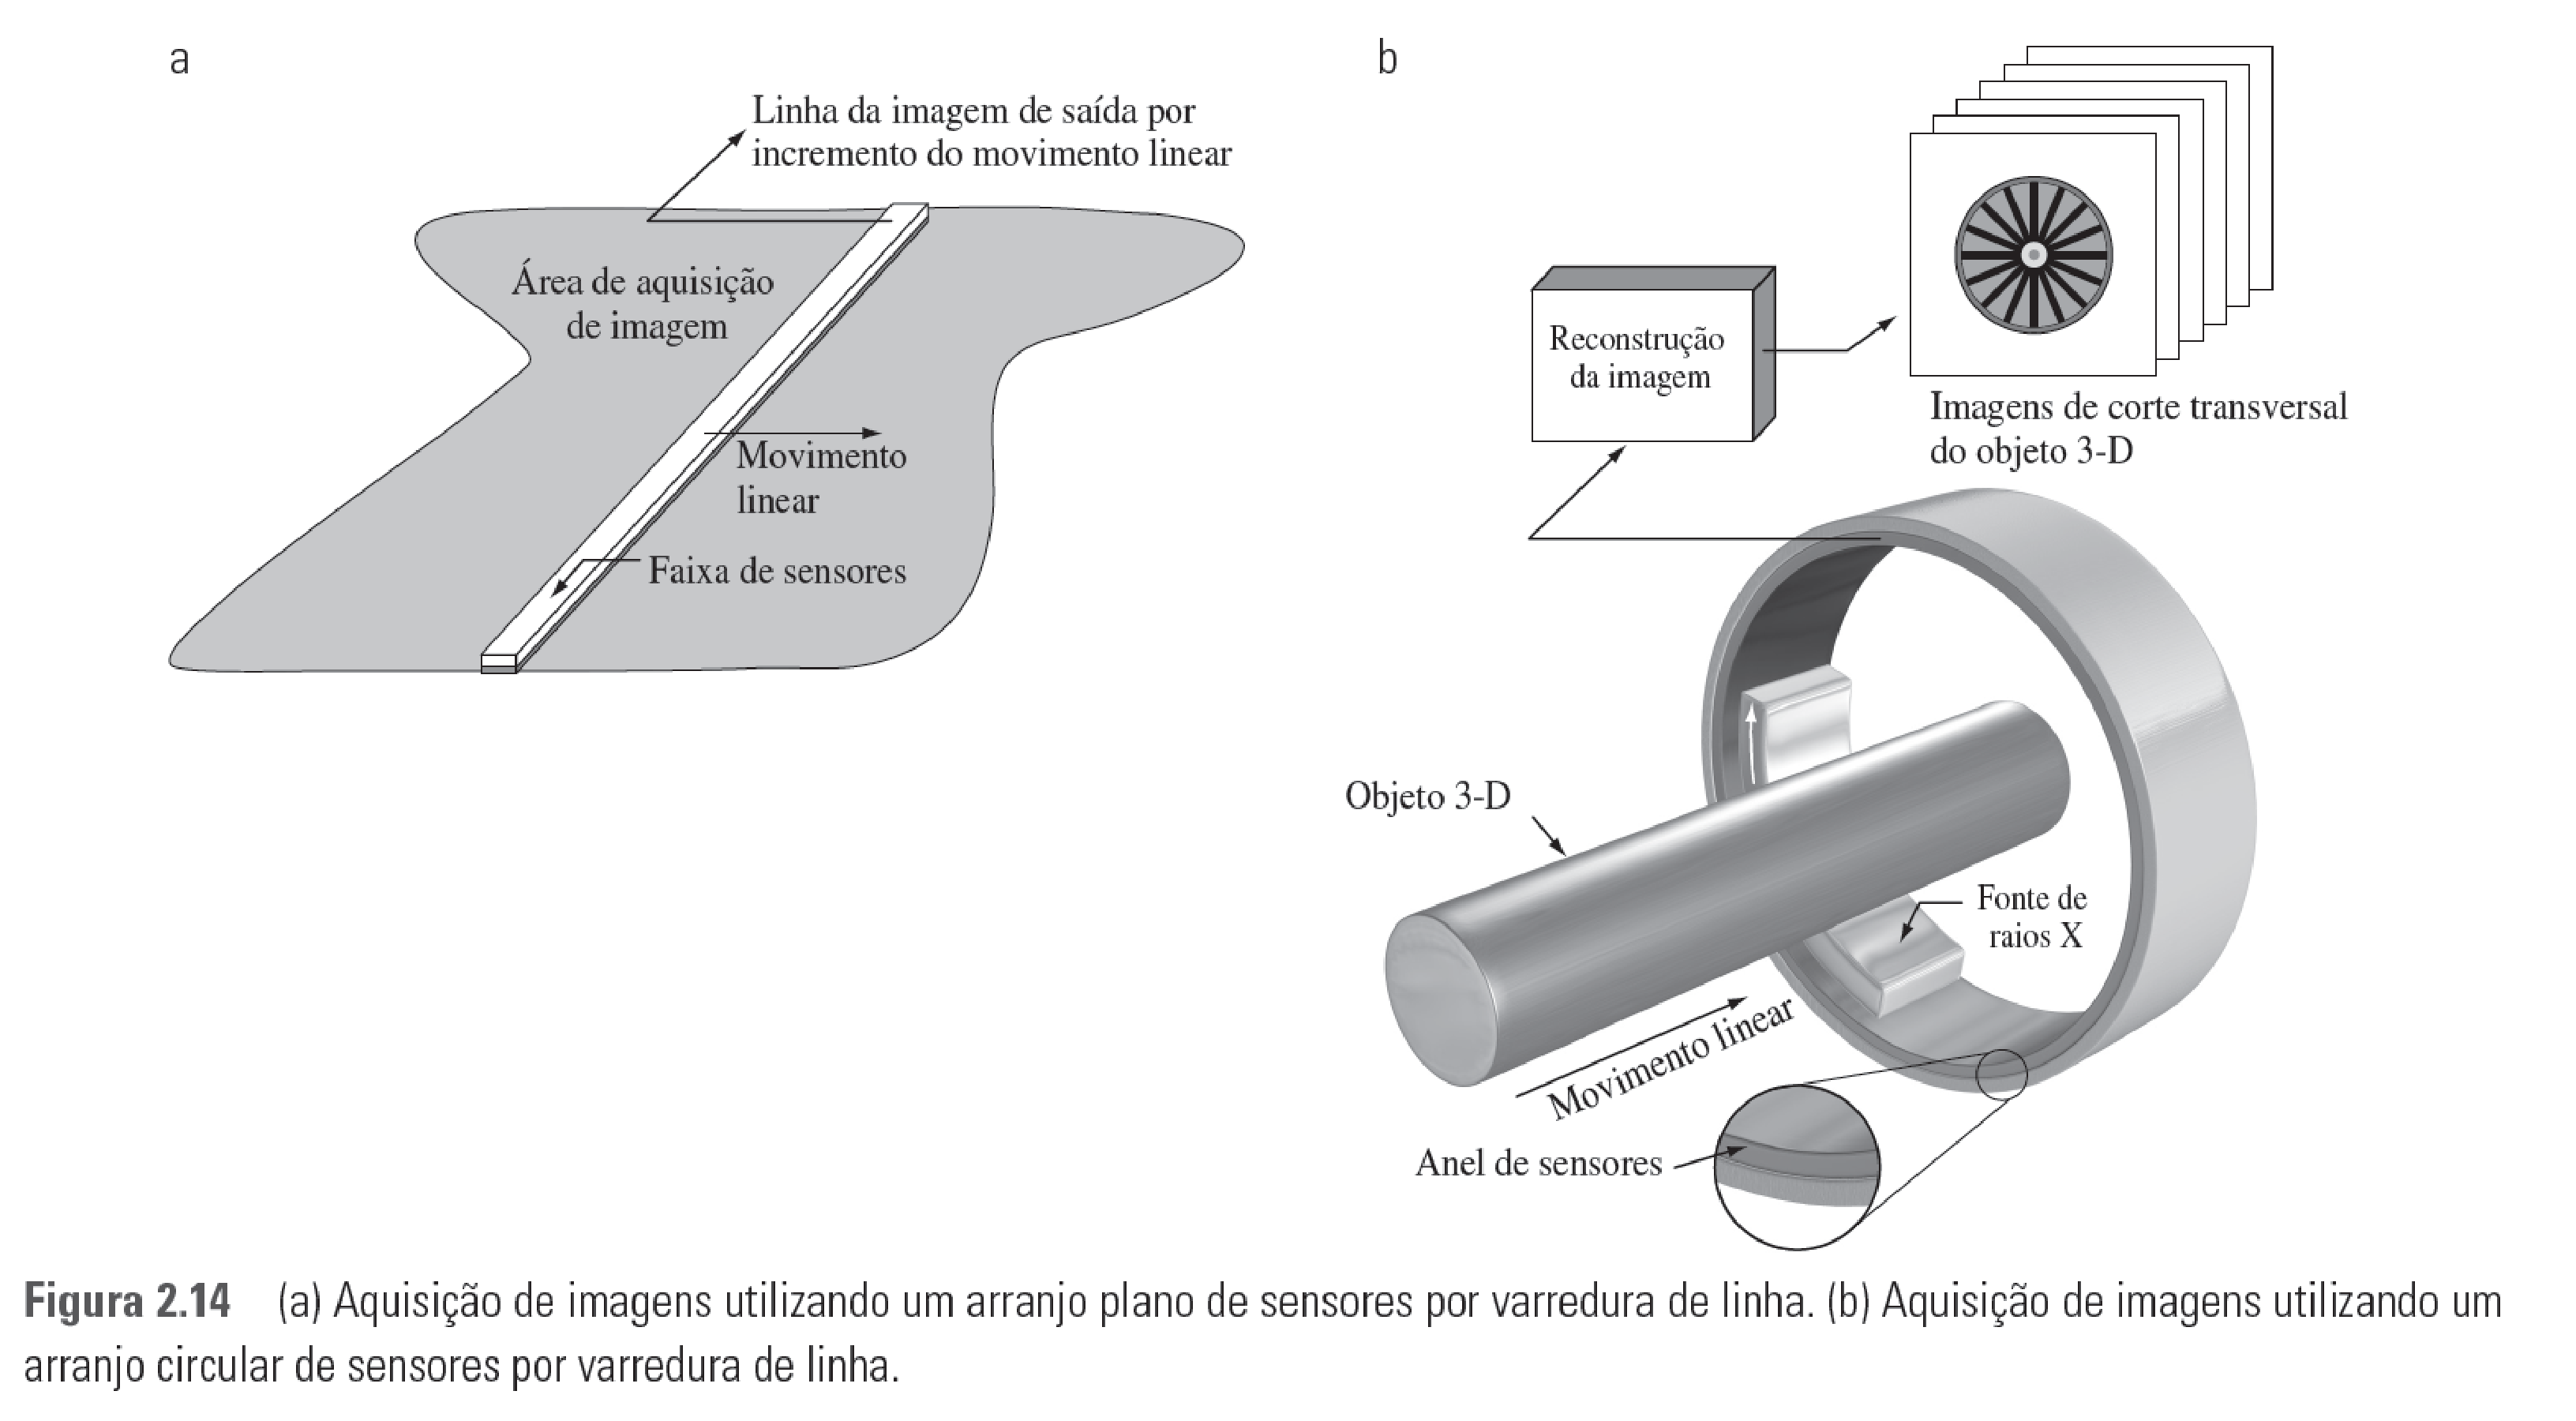
\includegraphics[width=.9\textwidth]{figs/fig0214}
            \end{center}
      \end{itemize}
   \end{slide}
   
   \begin{slide}[toc=]{Arranjos de foto sensores}
      \begin{itemize}[type=1]
         \item Arranjo matricial
            \begin{center}
               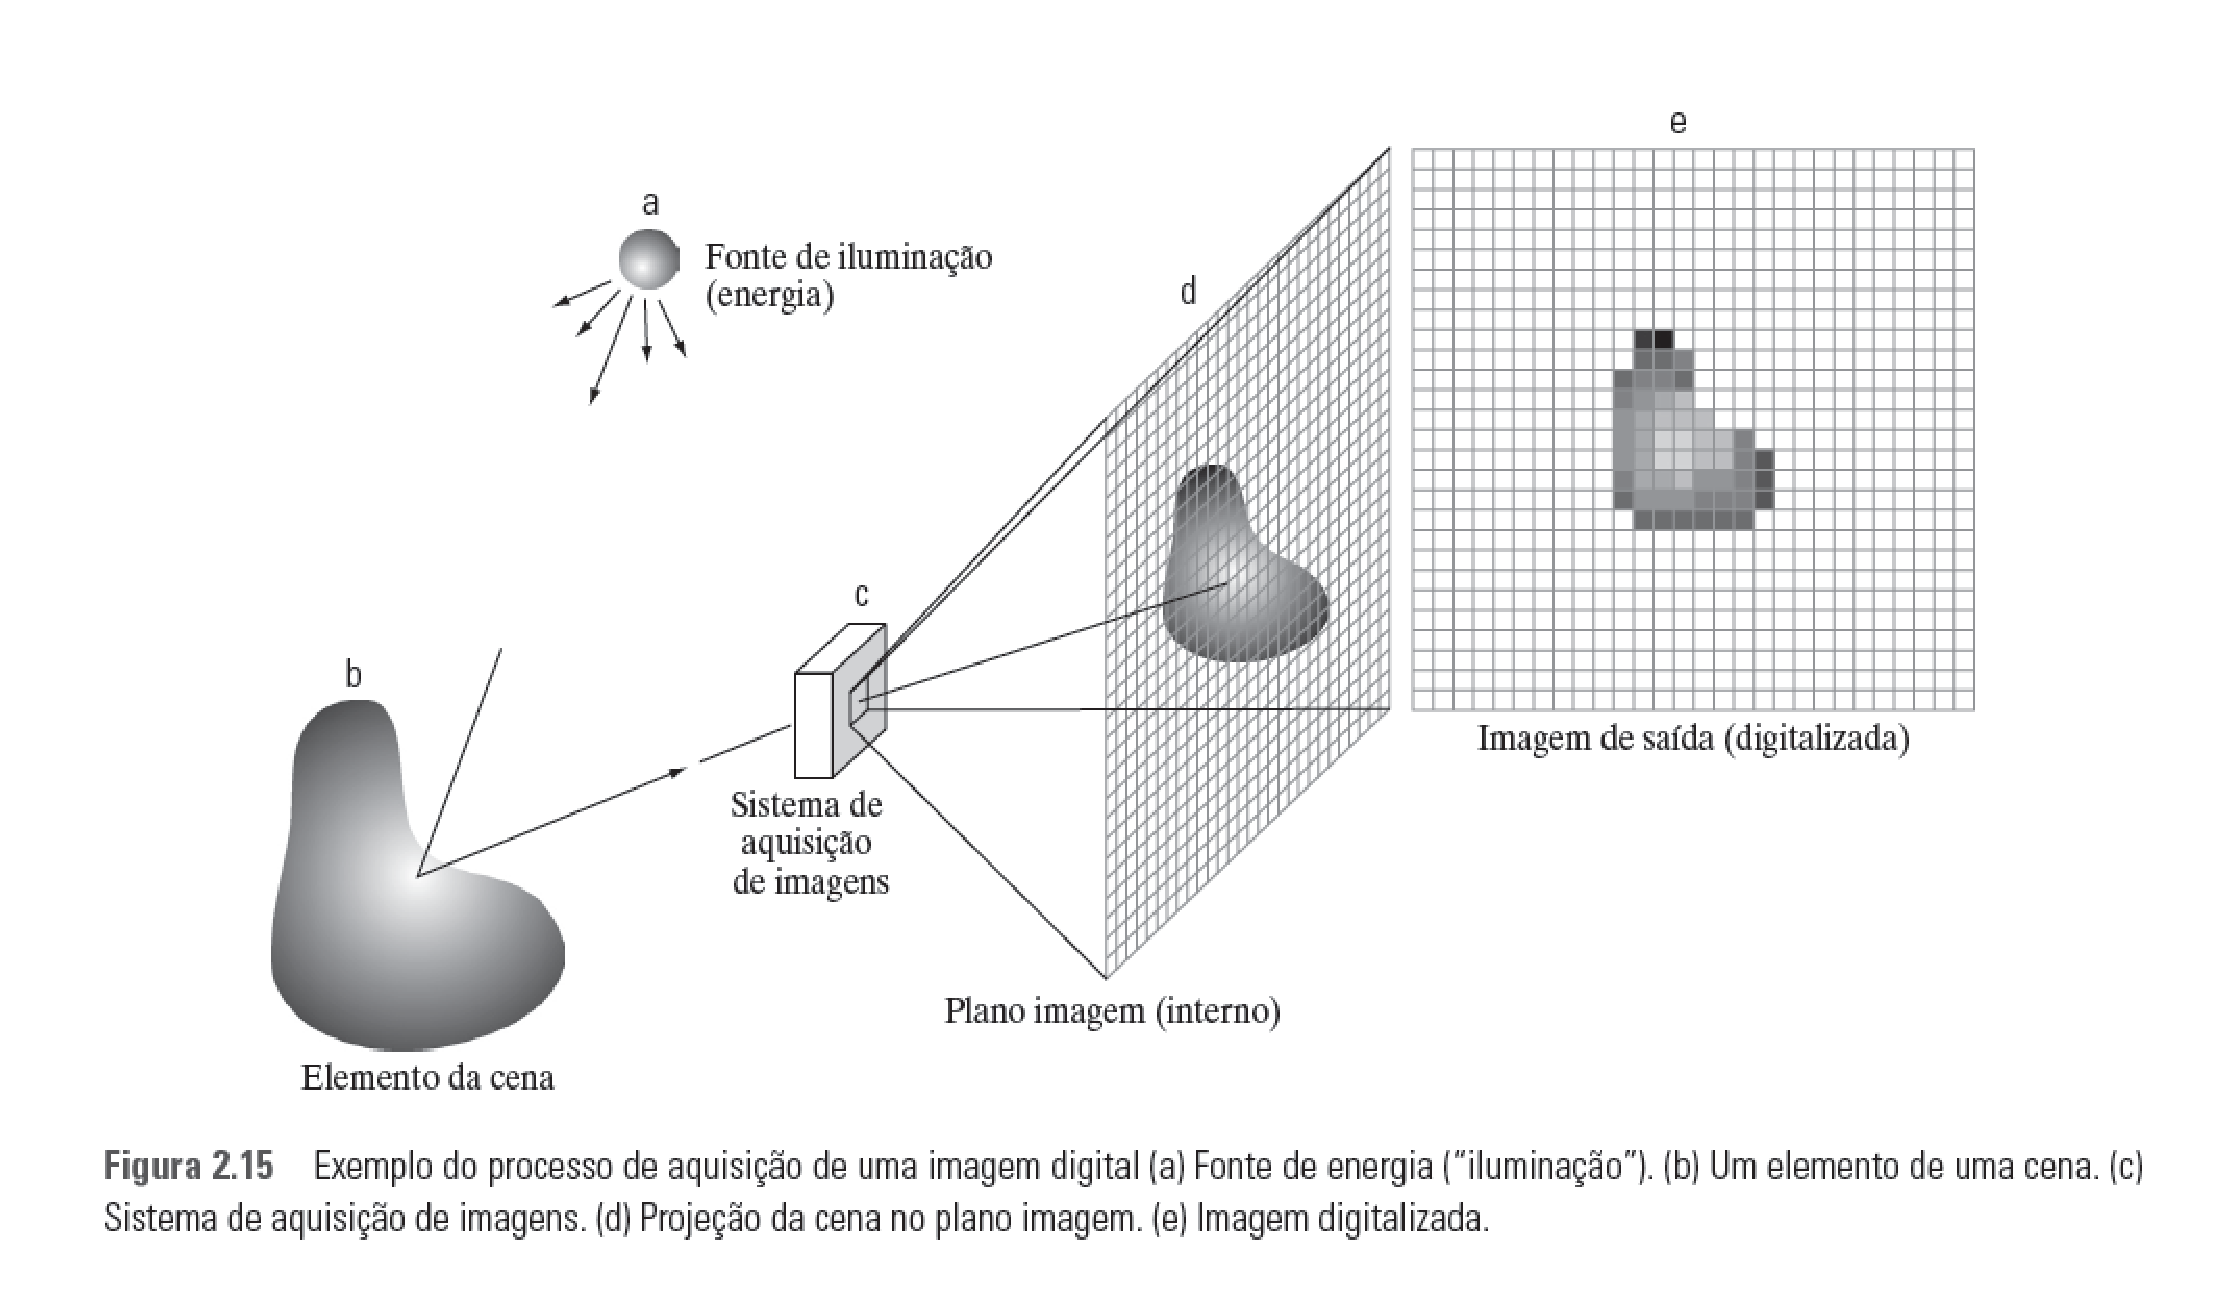
\includegraphics[width=.8\textwidth]{figs/fig0215}
            \end{center}
      \end{itemize}
   \end{slide}
   
    \begin{slide}[toc=]{Modelo de formação de imagem}
       \begin{equation*}
          f(x,y) = i(x,y)r(x,y) 
       \end{equation*}
      \begin{align*}
         0<&f(x,y)<\infty\\
         0<&i(x,y)<\infty\\
         0<&r(x,y)<1
      \end{align*}
      \begin{itemize}
       \item $f(x,y)$: intensidade
       \item $i(x,y)$: iluminação
       \item $r(x,y)$: refletância
      \end{itemize}
    \end{slide}

   \section[ slide = true ]{Amostragem e quantização de imagens}
   \begin{slide}[toc=]{Amostragem e quantização}
     \begin{itemize}
       \item O processo varia dependendo do arranjo de sensores utilizado
       \item Tudo o que foi abordado para o caso unidimensional é válido aqui
       \begin{itemize}
         \item Taxa de Nyquist
         \item Aliasing
       \end{itemize}
       \item Amostragem por varredura
        \begin{center}
          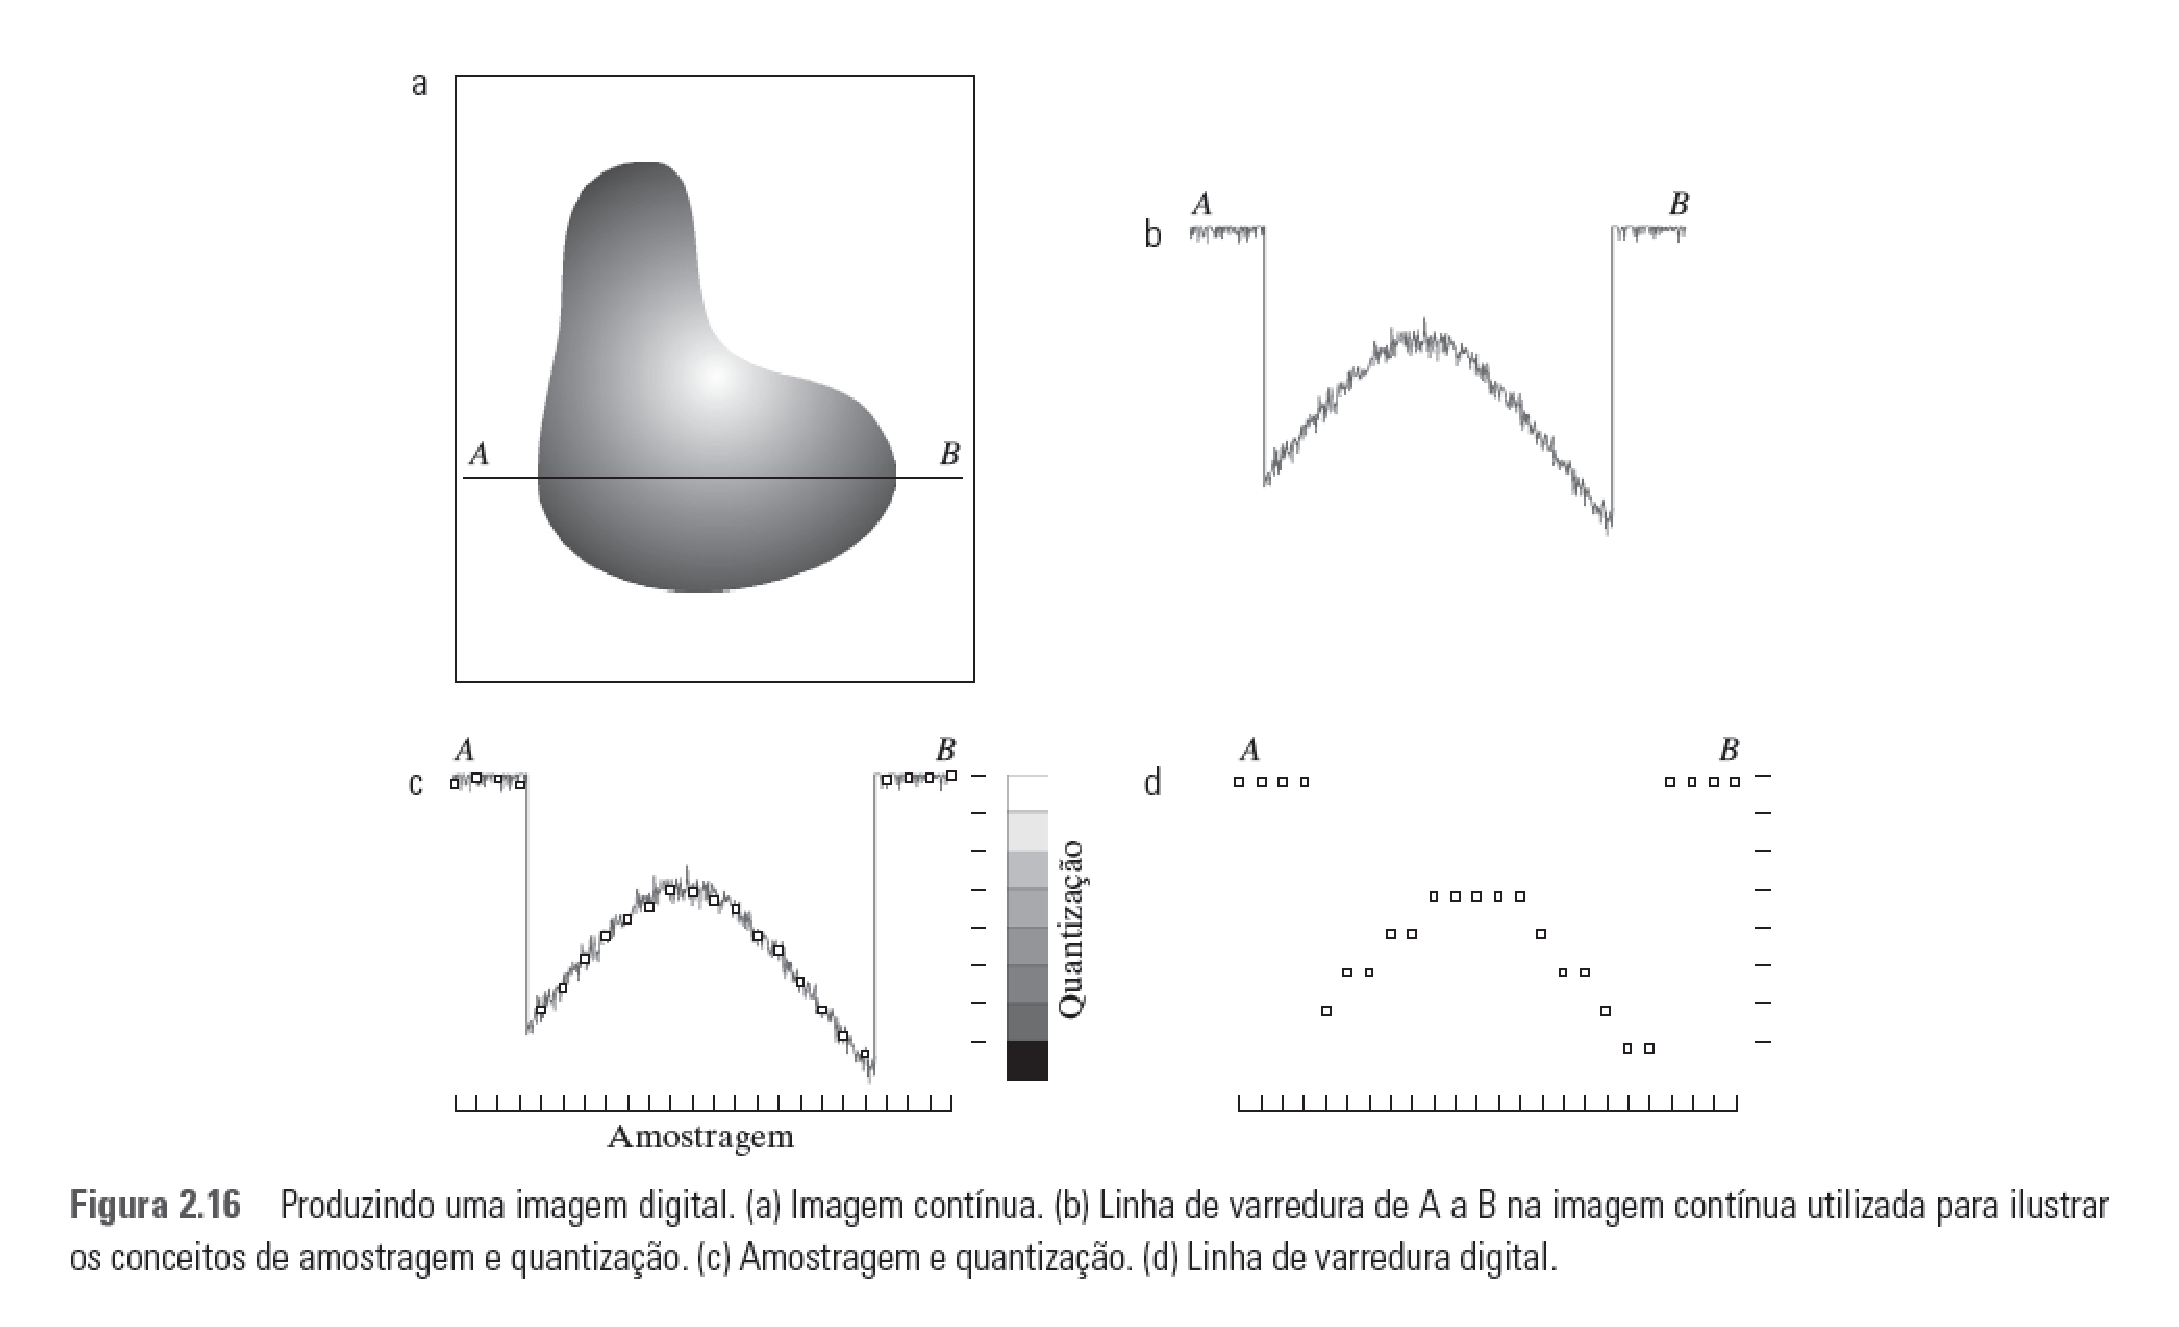
\includegraphics[width=0.6\textwidth]{figs/fig0216}
        \end{center}
     \end{itemize}
   \end{slide}
   
   \begin{slide}[toc=]{Amostragem e quantização}
     \begin{itemize}
        \item Amostragem por sensor matricial
        \begin{center}
          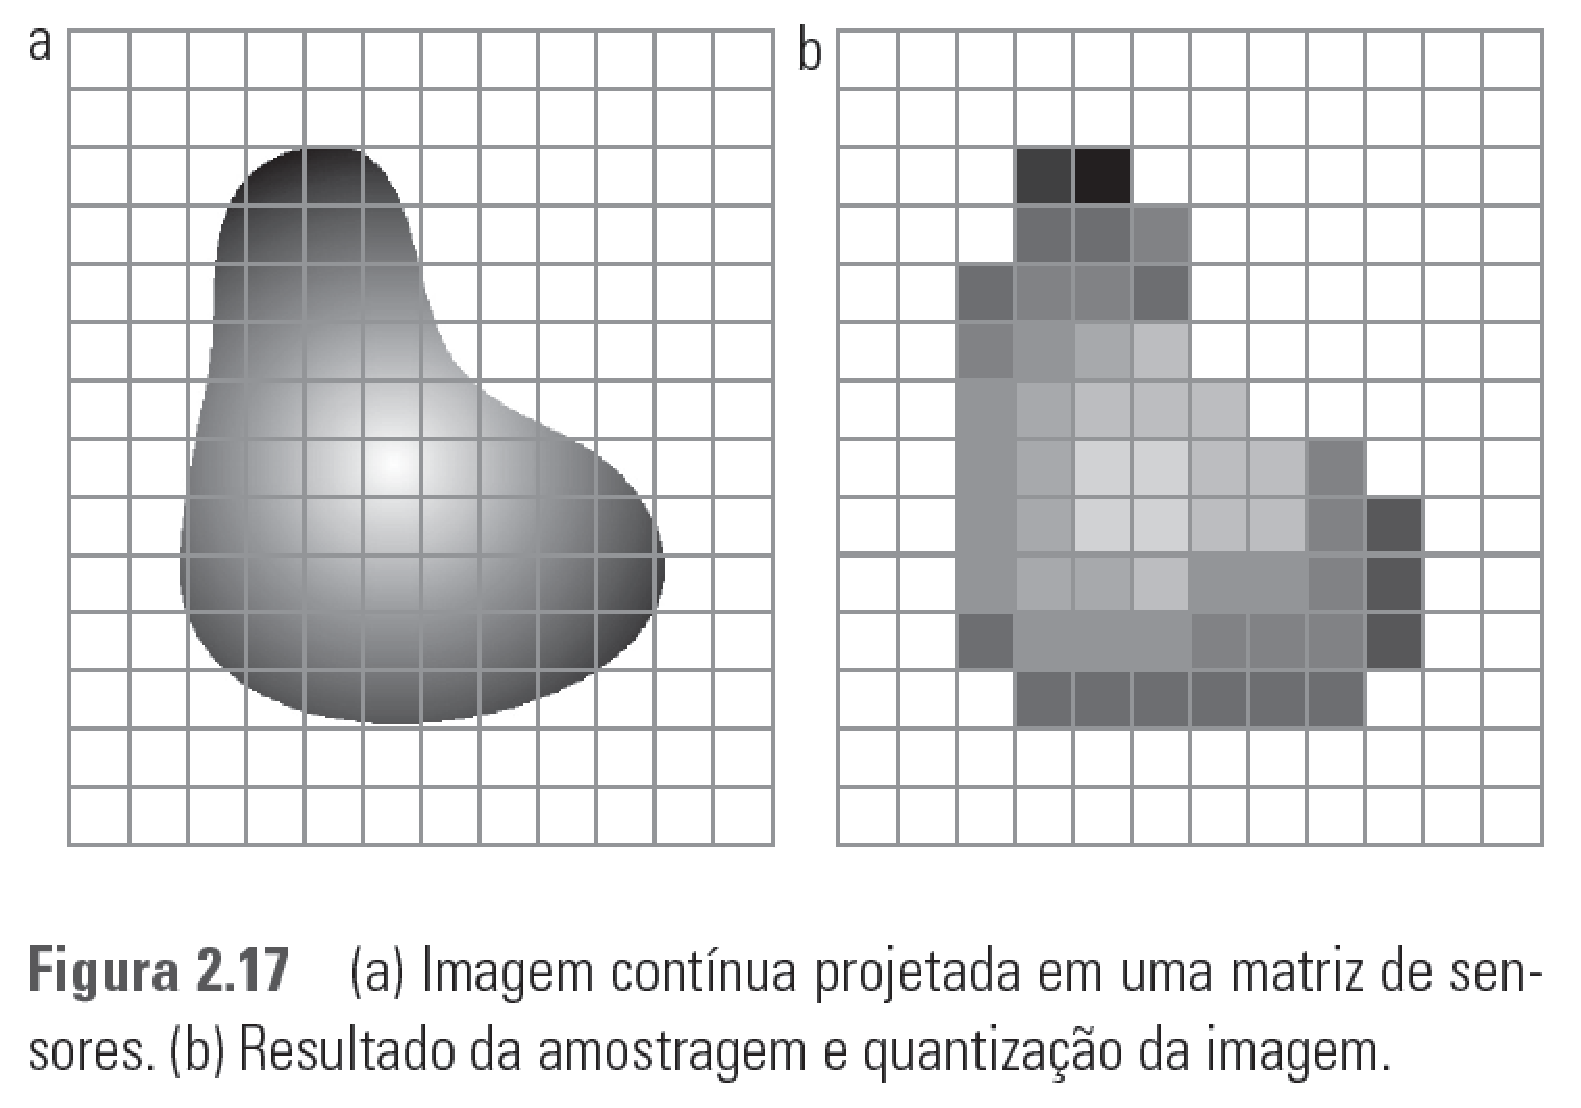
\includegraphics[width=0.6\textwidth]{figs/fig0217}
        \end{center}
     \end{itemize}
   \end{slide}
        
   \begin{slide}[toc=]{Representação de uma imagem digital}
        \begin{center}
          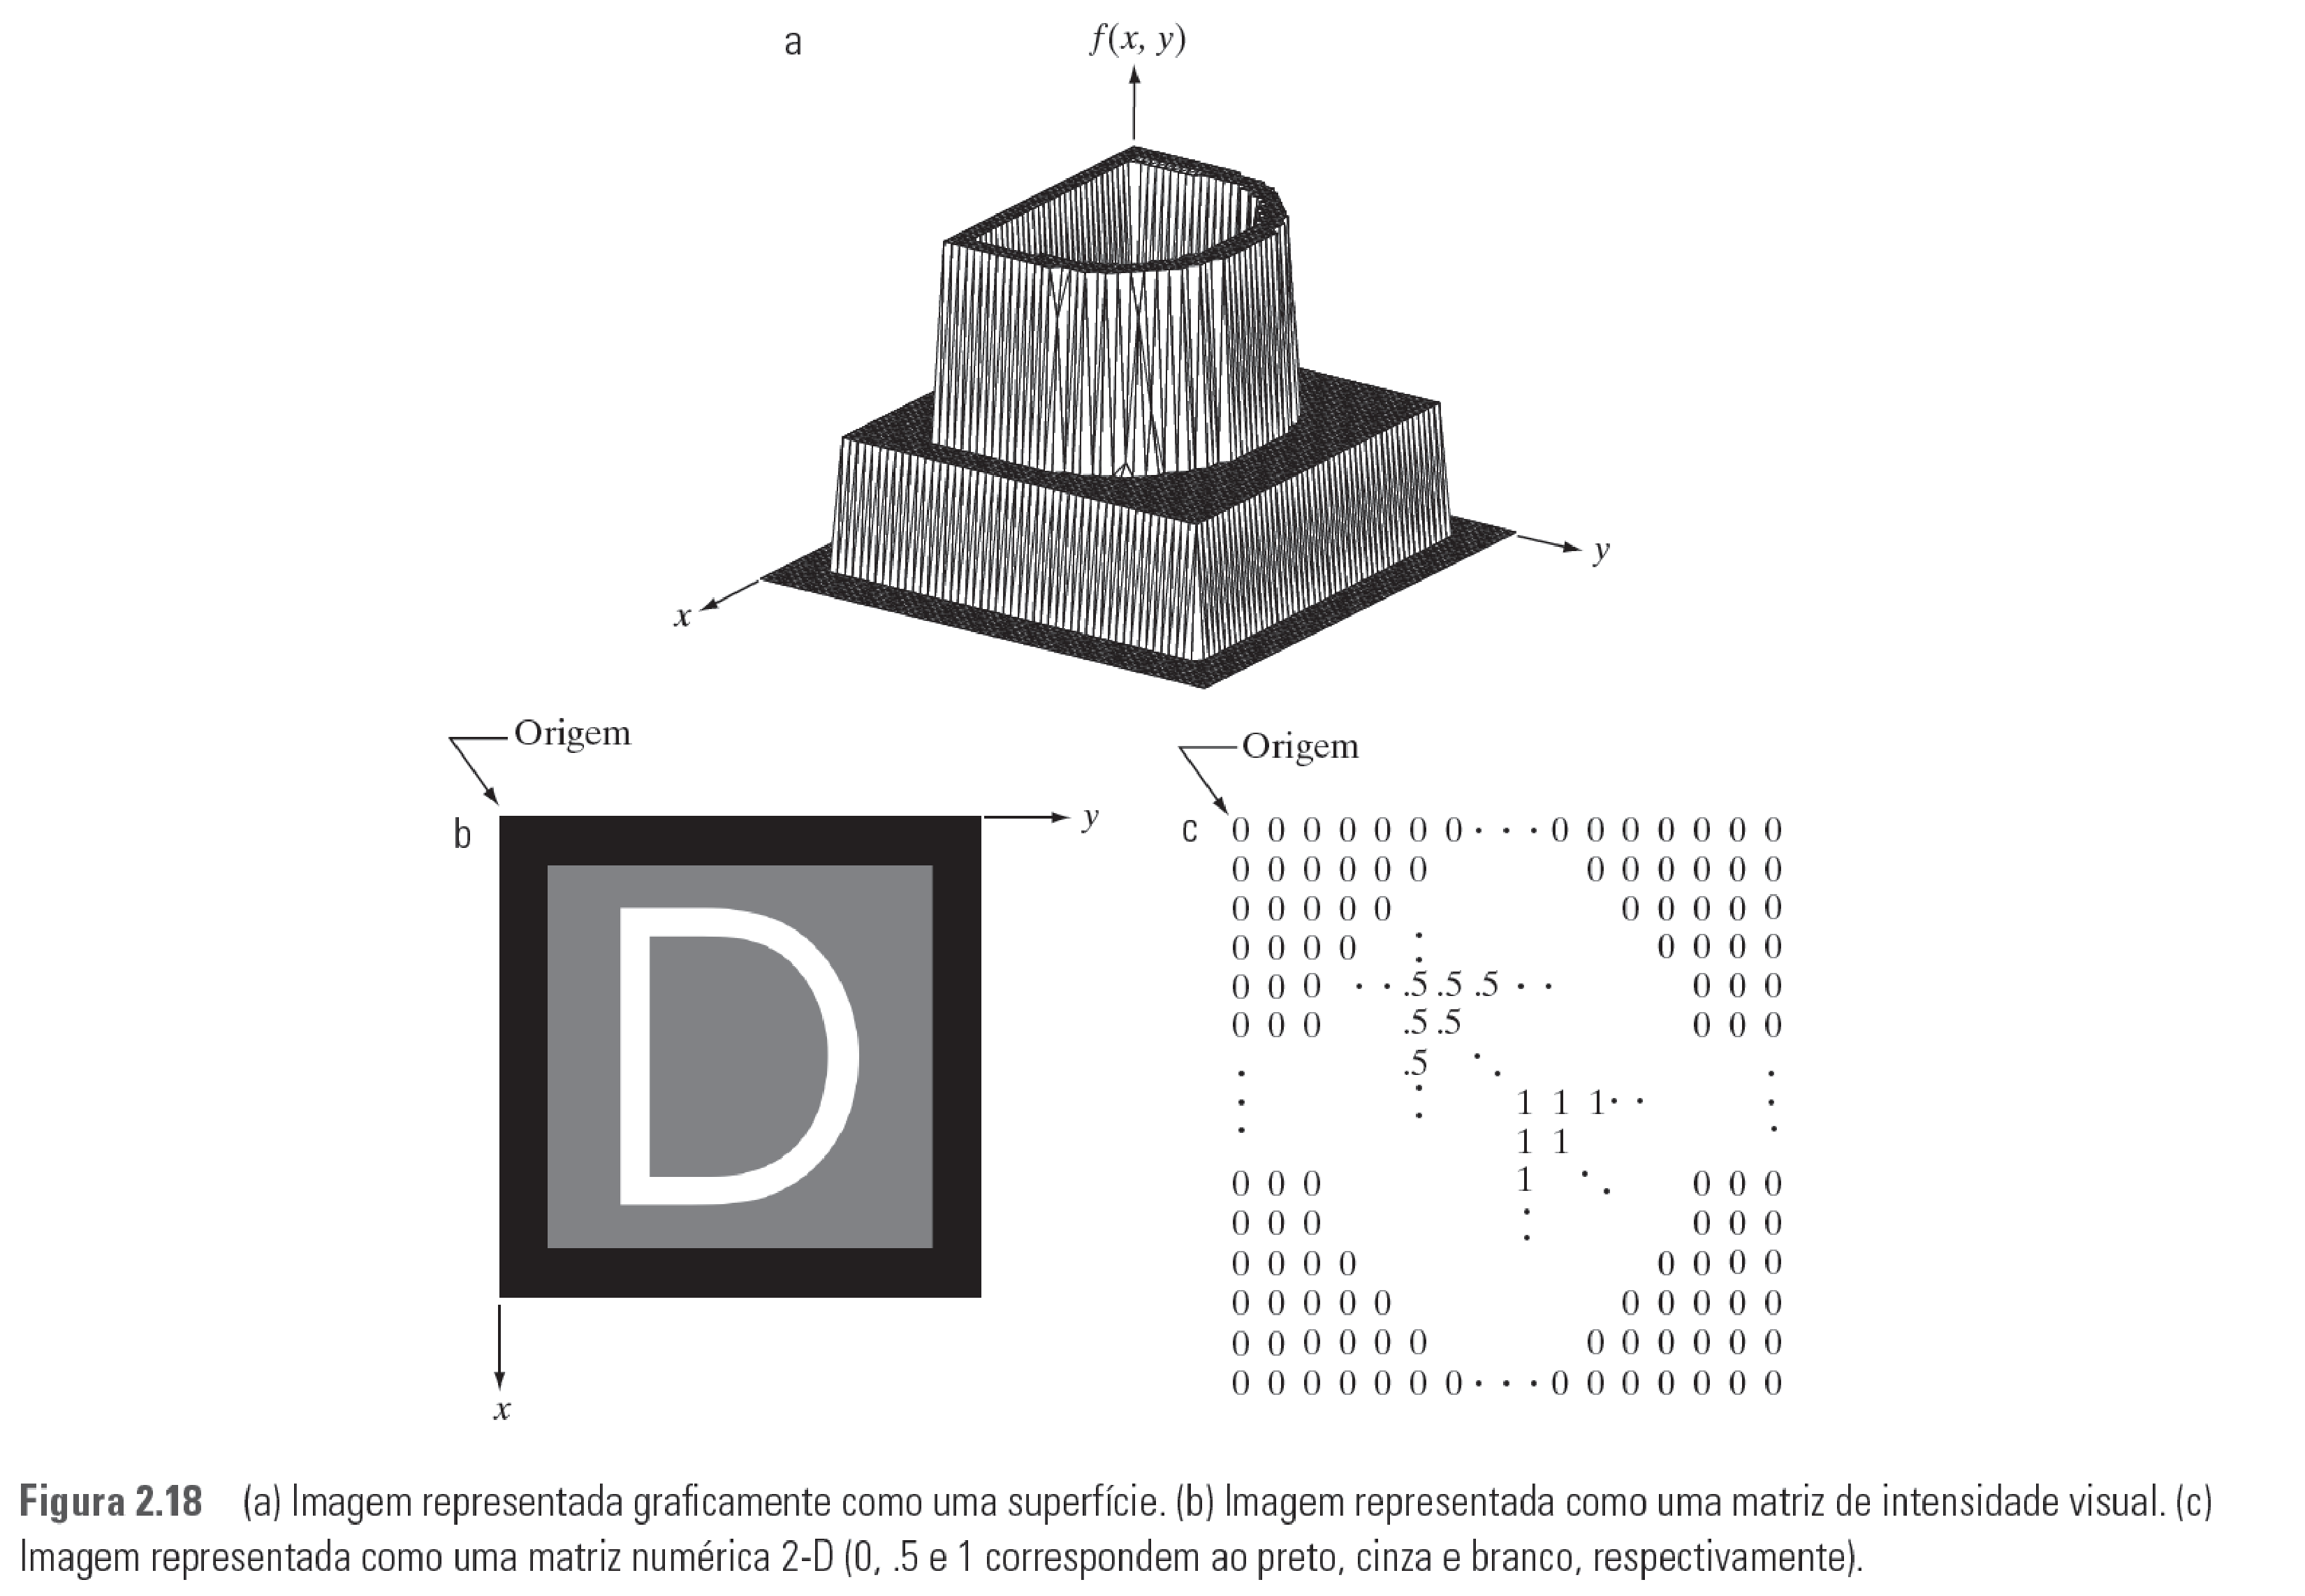
\includegraphics[width=.8\textwidth]{figs/fig0218}
        \end{center}
   \end{slide}
   
   \begin{slide}[toc=]{Resolução espacial}
   \begin{itemize}
    \item Razão entre quantidade de elementos por unidade de distância
    \item Exemplos: pontos por polegada (dpi), pares de linhas por milímetro, etc.
   \end{itemize}
        \begin{center}
          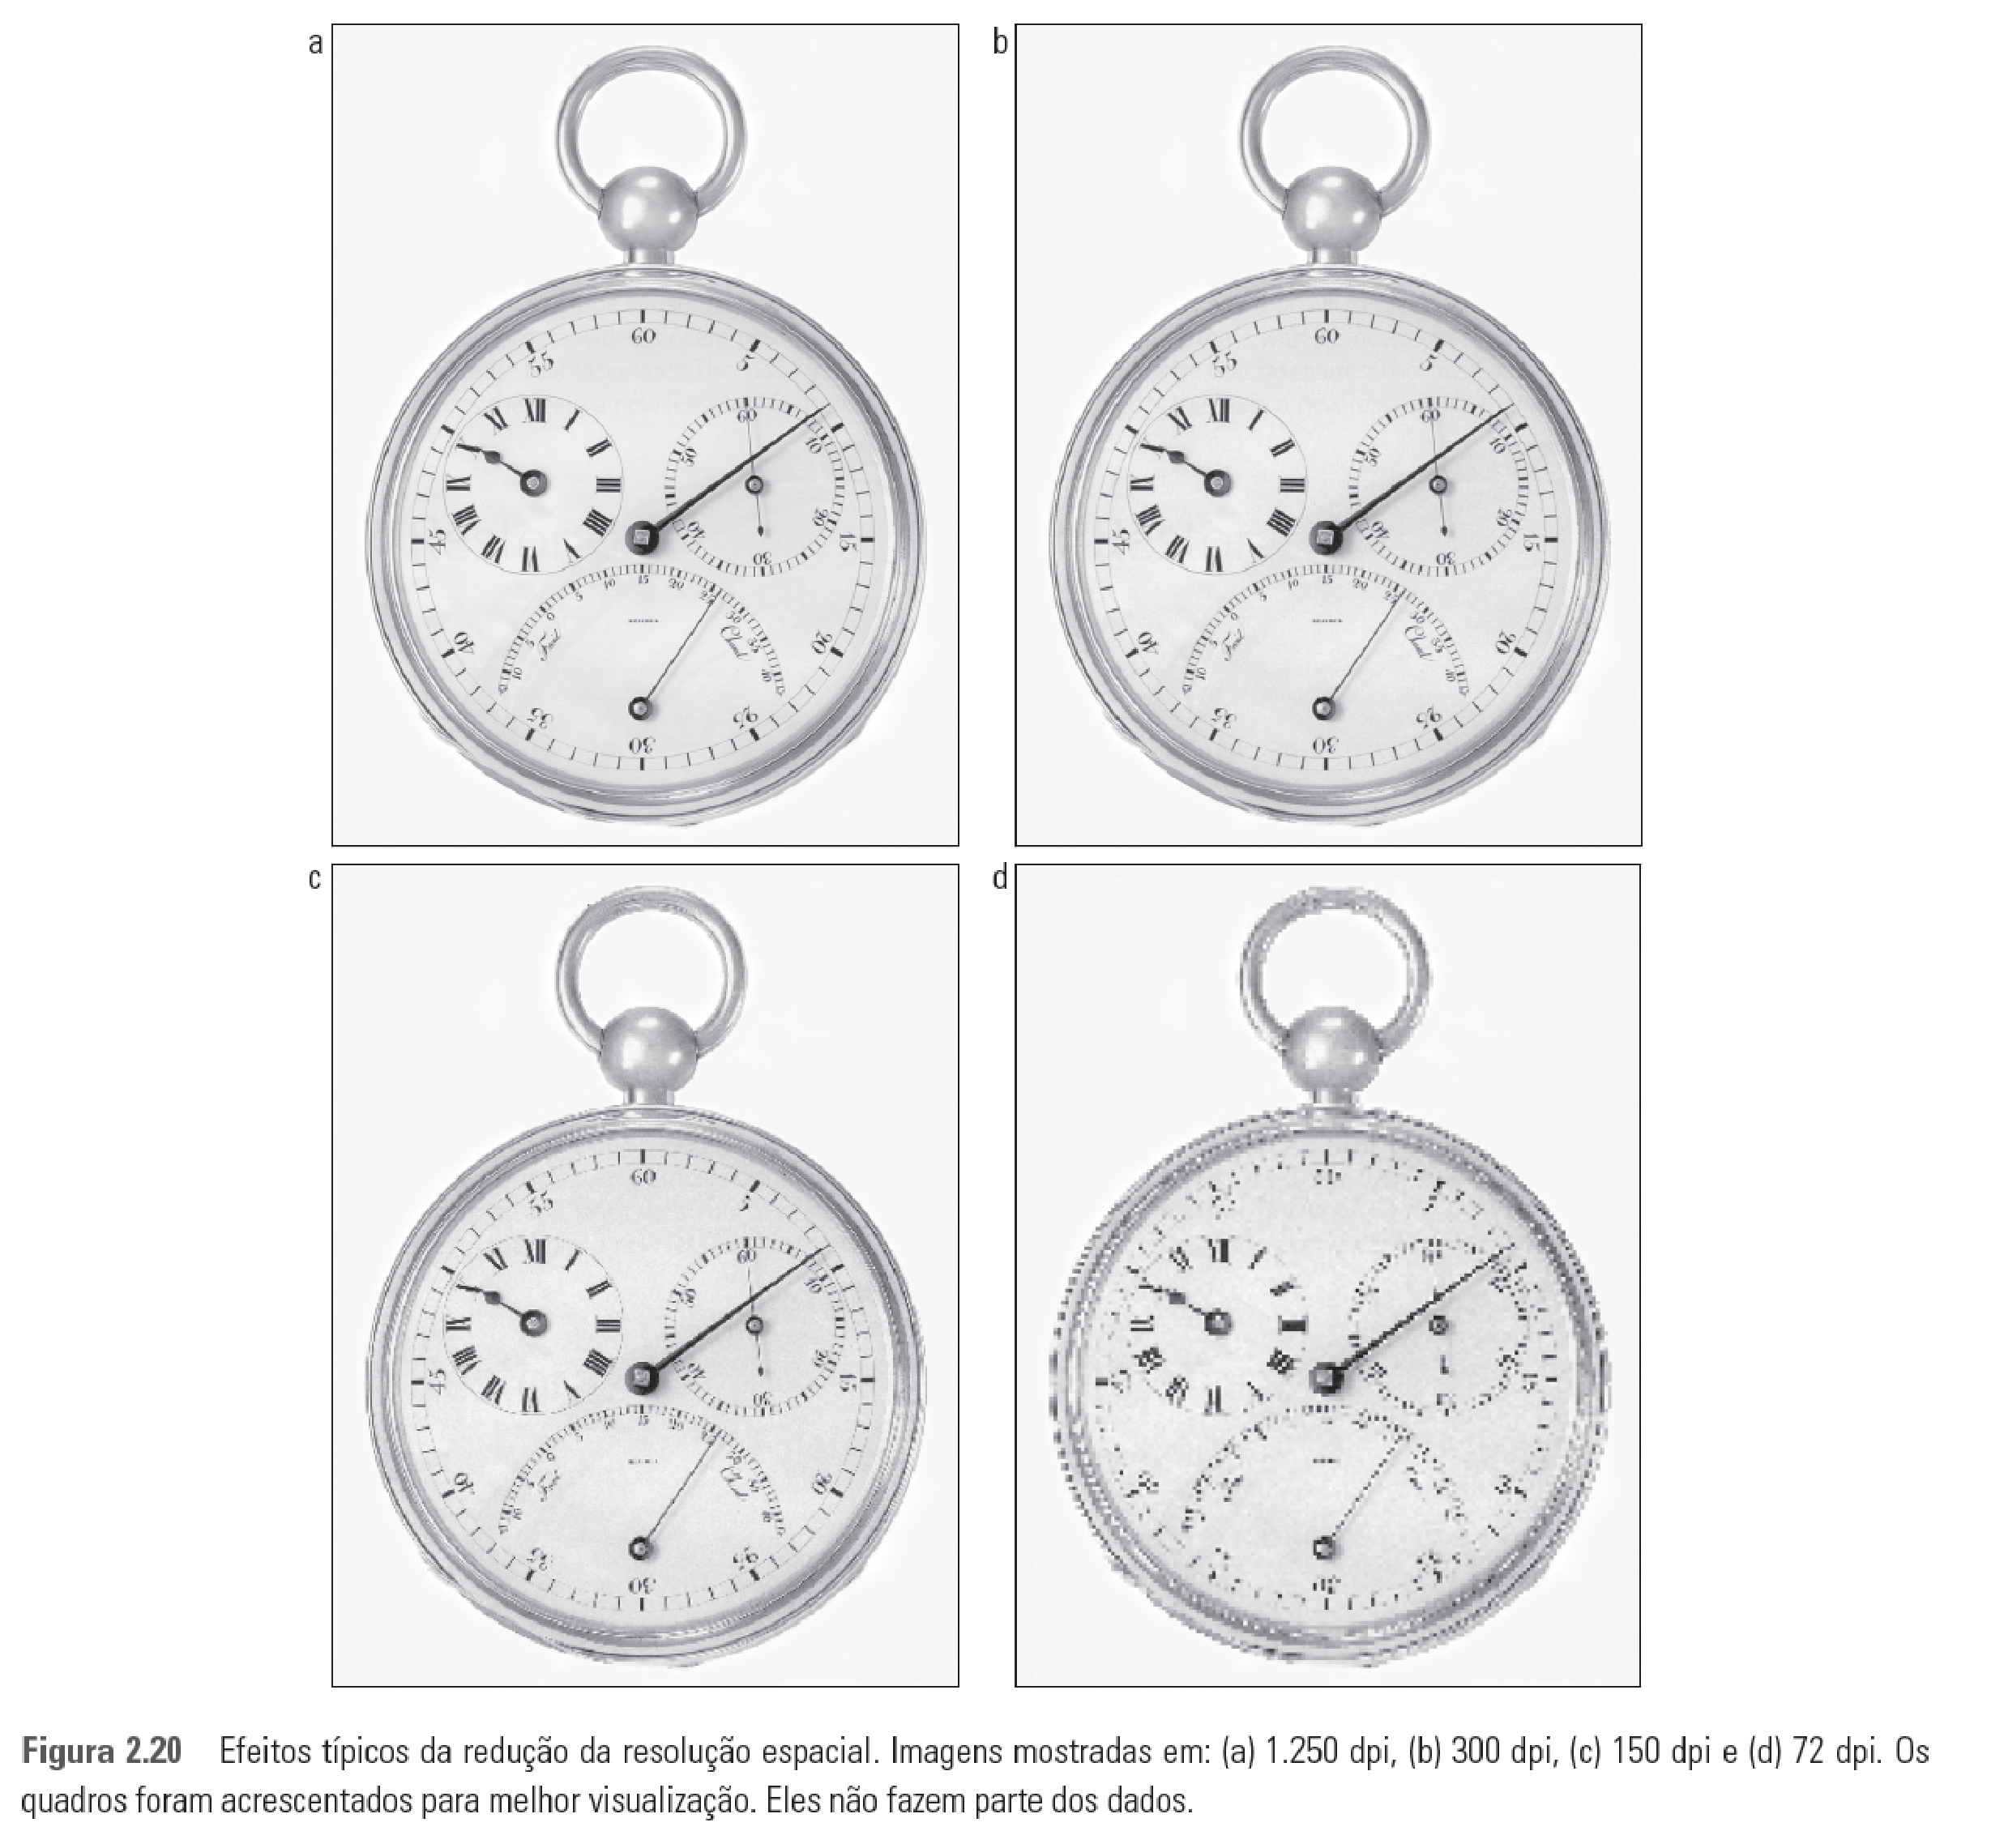
\includegraphics[width=0.5\textwidth]{figs/fig0220}
        \end{center}
   \end{slide}
   
   \begin{slide}[toc=]{Resolução de intensidade}
   \begin{itemize}
    \item Quantidade de níveis de intensidade diferentes
    \item Depende do número de bits usados na representação dos pixels
   \end{itemize}
        \begin{center}
          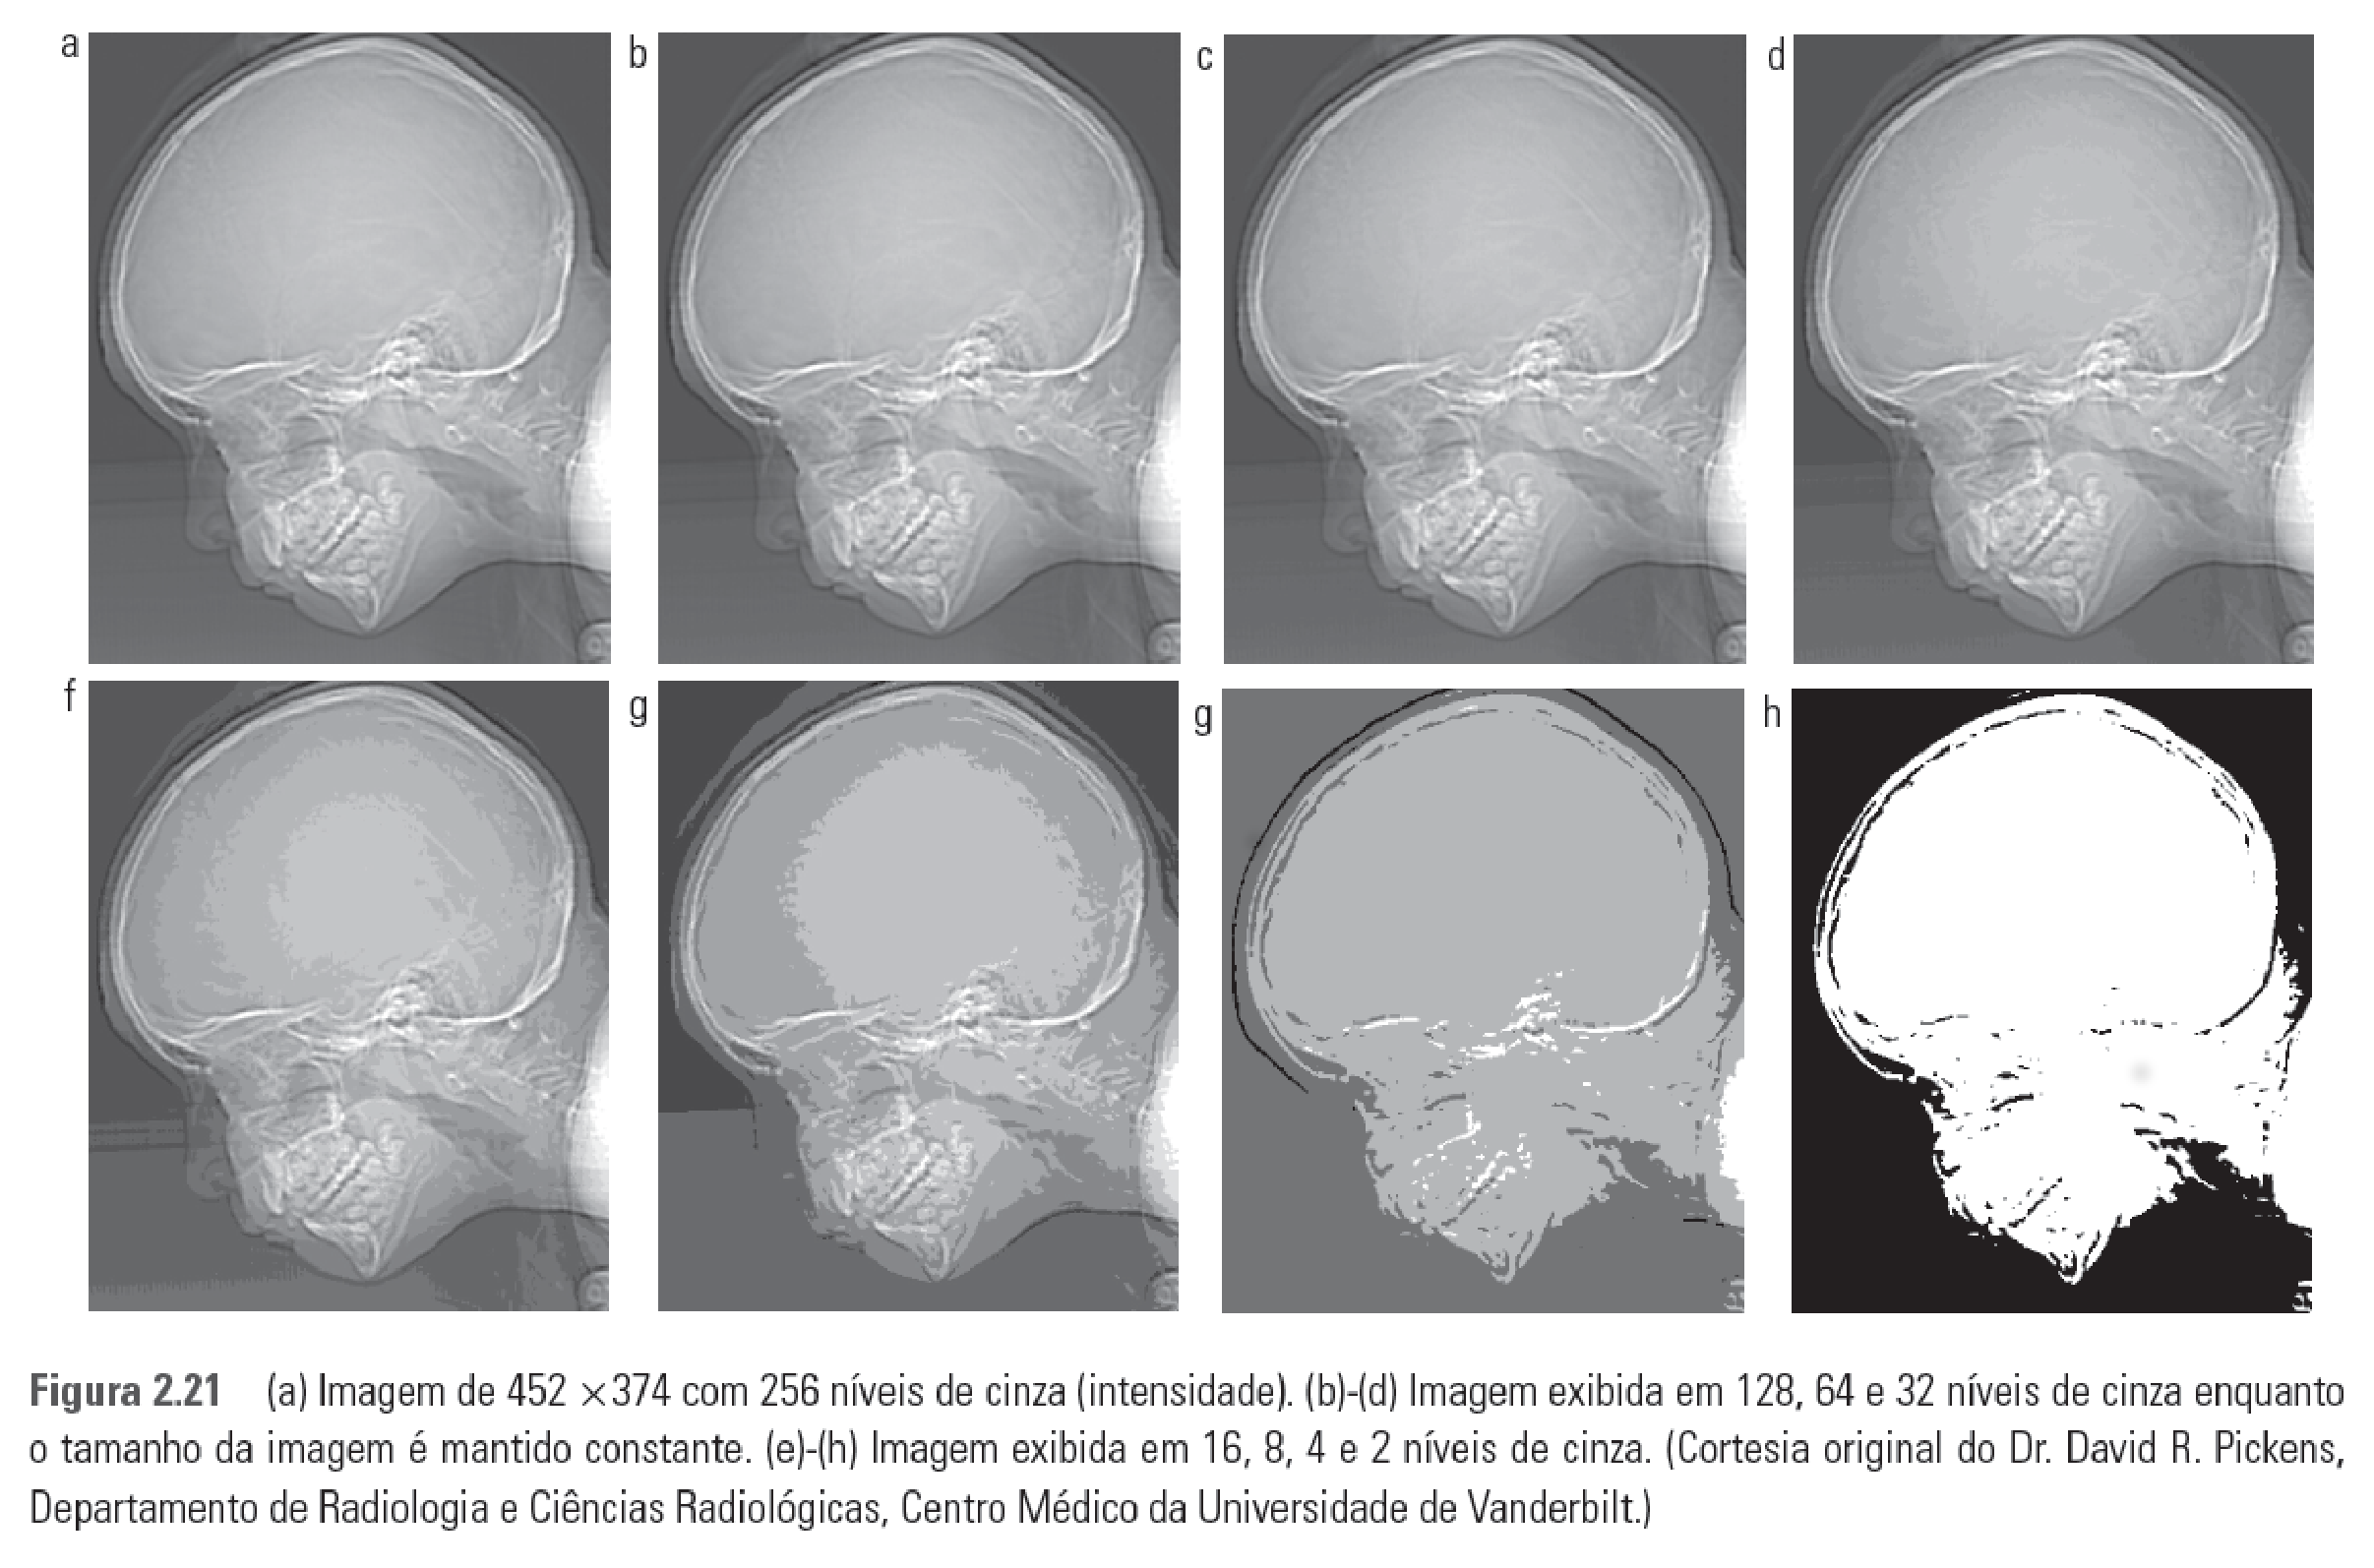
\includegraphics[width=0.7\textwidth]{figs/fig0221}
        \end{center}
   \end{slide}
\end{document}
